\section{Experiments}
\label{sec:experiments}

We evaluate SimPLe on a suite of Atari games from Atari Learning Environment (ALE) benchmark.
In our experiments, the training loop is repeated for 15 iterations, with $6400$ interactions with the environment collected in each iteration.
We apply a standard pre-processing for Atari games: a frame skip equal to 4, that is every action
is repeated 4 times and frames are down-scaled by a factor of 2.
%The task setup follows the standard ALE protocol~\cite{dqn}, with frame skipping, such that each action is repeated 4 times.  % and transformed to grayscale.
% Out of the 4 resulting frames, the last two were maxed per-pixel and used as input for the model.
% In order to speed-up the computations images has been down-scaled twice both horizontally and vertically; they have not been transformed to grayscale.
%%SL.1.22: Is the preprocessing the same as in Mnih et al? this kind of makes it sound like it's different
Because some data is collected before the first iteration of the loop,
altogether $6400 \cdot 16 = 102,400$ interactions with the Atari environment are used during training.
This is equivalent to $409,600$ frames from the Atari game (114 minutes in NTCS, 60 FPS).
All our code is available as part of the Tensor2Tensor library and it includes instructions on how
to run our experiments.\footnote{\url{https://github.com/tensorflow/tensor2tensor/tree/master/tensor2tensor/rl}} 
%%SL.1.22: say how much this corresponds to in real time?



%PM-22.01 here there is overlap with sect4
% For collecting the data from the real environment $env$ we are also using PPO which is using (and training) the same policy.
%%SL.1.22: can rephrase above as: 
At every iteration, the latest policy trained under the learned model is used to collect data in the real environment $\env$.
Due to vast difference between number of training data from simulated environment $env'$ and real environment $env$ -- 15M vs 100K
-- we believe that the impact of real data on policy is negligible.
%%SL.1.22: Perhaps the above discussion is a little more nuanced. Since we branch the model rollouts off of the real rollouts, their impact is likely *not* neglible, but it can also be discussed entirely in Section 5, and we can omit this discussion here
%PM22.01:Rember to set correctly, Possibly remove dopamine
 We evaluate our method on $26$ games selected on the basis of being solvable with existing state-of-the-art model-free deep RL algorithms\footnote{Specifically, for the final evaluation we selected games which achieved non-random results using our method or the Rainbow algorithm using $100$K interactions.}, which in our comparisons are Rainbow~\cite{rainbow} and PPO~\cite{ppo}.
 For Rainbow, we used the implementation from the Dopamine package and spent considerable
 time tuning it for sample efficiency.

For visualization of all experiments see the supplementary website
%\href{https://sites.google.com/view/modelbasedrlatari/home}{dedicated webpage}\footnote{\href{https://goo.gl/itykP8}{https://goo.gl/itykP8}}
\footnote{\url{https://goo.gl/itykP8}},
and for a summary see Figures \ref{fig:compare_dopamine} and  \ref{fig:compare_ppo}.
It can be seen that our method is more sample-efficient than a highly tuned Rainbow baseline
on almost all games, requires less than half of the samples on more than half of the games
and, on \freeway\, is more than 10x more sample-efficient. In terms of learning speed, our method outperforms PPO by an even larger margin.

%%SL.1.22: make sure the webpage is fully anonymous?
%%HM.1.23: it is

% \begin{figure*}[htbp]
% 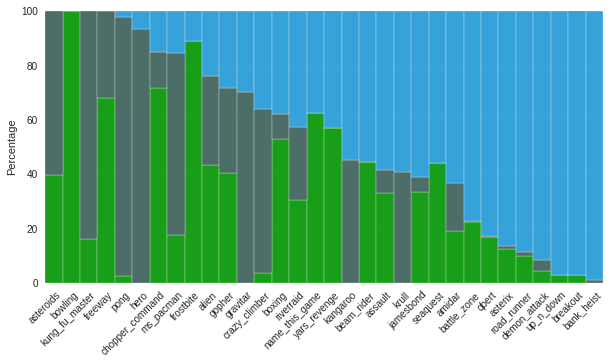
\includegraphics[width=0.95\textwidth]{figures/ppo_arxiv.png}
% \caption{Relative performance of  model-based agents trained with PPO using 100K frames (gray bars) compared to model-free agents trained with PPO using 40M frames (top line) and 1M frames (green bars).}
% \label{fig:graph_main_ppo}
% \end{figure*}


% \begin{figure*}[htbp]
% 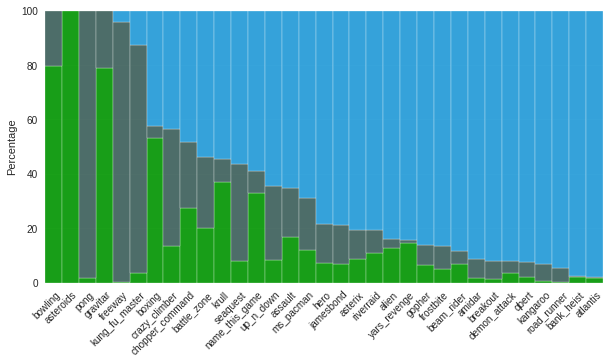
\includegraphics[width=0.95\textwidth]{figures/dqn_arxiv.png}
% \caption{Relative performance of  model-based agents trained with PPO using 100K frames (gray bars) compared to model-free agents trained with DQN (Dopamine) using 100M frames (top line) and 1M frames (green bars).}
% \label{fig:graph_main_ppo}
% \end{figure*}